\documentclass[12pt]{article}
  
  \usepackage[utf8]{inputenc}
  \usepackage[T1]{fontenc}
  \usepackage{geometry}
  \usepackage{graphicx}
  \geometry{a4paper}
  
  \usepackage[frenchb]{babel}
  
  \title{Assignment :B5}
  \author{Roll no : 4430}
  \date{}
  
  \begin{document}
  \maketitle
  
\section{Problem Definition}
Code generation using DAG /labelled tree.


\section{Learning Objectives}

\begin{enumerate}
\item To understand concept of DAG or labelled tree.
\item To learn code generation.
\end{enumerate}

\section{Learning Outcome}
\begin{enumerate}
\item Able to understand DAG or labelled tree.
\item Able to generate code using DAG or labelled tree
\end{enumerate}


\section{Software and hardware requirements.}
\begin{enumerate}
\item C++ Compiler
\item 64-bit open source operating system(fedora).
\item Eclipse
\end{enumerate}  

\section{Mathematical Model}
Let S be the system of solution of given problem statement.\\
s=\{s,e,X,Y,F,DD,NDD,Su,Fu \}\\\\
where,\\
s=start state ;\\
such that, y=\{\}\\\\
e=end state;\\
such that, y=\{Code is generated.\}\\

X=set of input ;\\
such that X=\{x1,x2\}\\
x1=operator\\
operator= + ,-, *, /\\
x2=operands\\
operands [a - z][A - Z]\\
Y=set of output ;\\
such that Y=\{I\} and I is intermediate code generated.\\\\
F=set of function ;\\
such that F=\{f1,f2,f3\}\\
where,\\
f1=function to insert root and respective nodes to tree.\\
\{node | node $\in$ X\}\\
f2=function to find label of leaf nodes.\\
f3=function to find label of interior nodes.\\
f4=function to initialize stack content.\\
{stack = 0}\\
f5=function to print in-order nodes of tree.\\
f6=function to print assembly code w.r.t label.\\
f7=function to delete all nodes of tree.\\

DD=Deterministic data\\
\{x1,x2\}\\\\
NDD=Non-deterministic data\\
=\{Assembly code generated.\}\\
Su=Success\\
Assembly code is generated and it is according to given input.\\\\
Fu=Failure\\
1.Assembly code is not generated\\
2.Invalid expression as input.\\\\

\section{Concept Related Theory}
\subsection{Directed acyclic graph}

In mathematics and computer science, a directed acyclic graph, is a directed
graph with no directed cycles. That is, it is formed by a collection of vertices and
directed edges, each edge connecting one vertex to another, such that there is no
way to start at some vertex v and follow a sequence of edges that eventually loops
back to v again.\\

A directed acyclic graph (DAG!) is a directed graph that contains no cycles.
A rooted tree is a special kind of DAG and a DAG is a special kind of directed
graph. For example, a DAG may be used to represent common subexpressions in
an optimising compiler.\\

DAGs may be used to model many different kinds of information. The reachability
relation in a DAG forms a partial order, and any finite partial order may
be represented by a DAG using reachability. A collection of tasks that must be
ordered into a sequence, subject to constraints that certain tasks must be performed
earlier than others, may be represented as a DAG with a vertex for each task
and an edge for each constraint ; algorithms for topological ordering may be used
to generate a valid sequence. Additionally, DAGs may be used as a space-efficient
representation of a collection of sequences with overlapping subsequences. DAGs
are also used to represent systems of events or potential events and the causal
relationships between them. DAGs may also be used to model processes in which
data flows in a consistent direction through a network of processors, or states of a
repository in a version-control system.\\
Applications of DAG :\\
1) Path Algorithms\\
2) Scheduling\\
3) Data Processing Networks\\
4) Causal Structure\\
5) Data Compression\\
Each instruction in triples presentation has three fields : op, arg1, and arg2.The
results of respective sub-expressions are denoted by the position of expression.
Triples represent similarity with DAG and syntax tree. They are equivalent to
DAG while representing expressions.\\\\

\subsection{Assembly Code}
An assembly language (or assembler language) is a low-level programming language
for a computer, or other programmable device, in which there is a very strong
(generally one-to-one) correspondence between the language and the architectures
machine code instructions. Each assembly language is specific to a particular computer
architecture, in contrast to most high-level programming languages, which
are generally portable across multiple architectures, but require interpreting or
compiling.\\

Assembly language is converted into executable machine code by a utility program
referred to as an assembler ; the conversion process is referred to as assembly,
or assembling the code.\\

Assembly language uses a mnemonic to represent each low-level machine instruction
or operation. Typical operations require one or more operands in order
to form a complete instruction, and most assemblers can therefore take labels,
symbols and expressions as operands to represent addresses and other constants,
freeing the programmer from tedious manual calculations. Macro assemblers include
a macroinstruction facility so that (parametrized) assembly language text
can be represented by a name, and that name can be used to insert the expanded
text into other code. Many assemblers offer additional mechanisms to facilitate
program development, to control the assembly process, and to aid debugging.\\


\section{State Diagram }
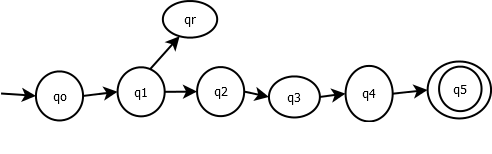
\includegraphics{a5state}

where,\\
q0 = start state.\\
q1 = accept labelled strict binary tree.\\
q2 = label leaf nodes and interior nodes.\\
q3 = display inorder of nodes.\\
q4 = display generated assembly code.\\
q5 = end state.\\
qr = rejection state.\\

\section{Program Code and Output}
\begin{verbatim}
#include<stdlib.h>
#include<iostream>
using namespace std;

/* We will implement DAG as Strictly Binary Tree
 where each node has zero or two children */

struct bin_tree 
{
char data;
int label;
struct bin_tree *right, *left;
};
typedef bin_tree node;

class dag
{
private:
/* R is stack for storing registers */
int R[10];
int top;

/* op will be used for opcode name w.r.t.
 arithmetic operator e.g. ADD for + */
char *op;

public: 

void initializestack(node *root)
{
/* value of top = index of topmost element of
 stack R = label of Root of tree(DAG) minus one */
    top=root->label - 1;

    /* Allocating Stack Registers */
    int temp=top;
    for(int i=0;i<=top;i++)
       {
          R[i]=temp;
          temp--;
       }
}

/* insertnode() and insert() functions are for adding nodes to tree(DAG) */

void insertnode(node **tree,char val)
{
node *temp = NULL;

if(!(*tree))
    {
        temp = (node *)malloc(sizeof(node));
        temp->left = temp->right = NULL;
        temp->data = val;
        temp->label=-1;
        *tree = temp;
    }
}

void insert(node **tree,char val)
{
    char l,r;
    int numofchildren;

    insertnode(tree, val);

    cout << "\nEnter number of children of " << val <<" :";
    cin >> numofchildren;

  if(numofchildren==2)
   {
    cout << "\nEnter Left Child of " << val <<" :";
    cin >> l;
    insertnode(&(*tree)->left,l);

    cout << "\nEnter Right Child of " << val <<" :";
    cin >> r;
    insertnode(&(*tree)->right,r);
   
    insert(&(*tree)->left,l);
    insert(&(*tree)->right,r);
   }
}

/* findleafnodelabel() will find out the label of leaf nodes of tree(DAG) */

void findleafnodelabel(node *tree,int val)
{

if(tree->left != NULL && tree->right !=NULL)
{
findleafnodelabel(tree->left,1);
findleafnodelabel(tree->right,0);
}

else
{
tree->label=val;
}

}

/* findinteriornodelabel() will find out 
the label of interior nodes of tree(DAG) */

void findinteriornodelabel(node *tree)
{
if(tree->left->label==-1) 
{
findinteriornodelabel(tree->left);
}

else if(tree->right->label==-1)
{
findinteriornodelabel(tree->right);
}

else
{

if(tree->left != NULL && tree->right !=NULL)
{

if(tree->left->label == tree->right->label)
{

tree->label=(tree->left->label)+1;
}

else
{

if(tree->left->label > tree->right->label)
{
tree->label=tree->left->label;
}
else
{
tree->label=tree->right->label;
}
}
}
}
}

/* function print_inorder() will print inorder of nodes.
 Here we are also printing label of each node of tree(DAG) */

void print_inorder(node * tree)
{
    if (tree)
    {
        print_inorder(tree->left);
        cout << tree->data <<" with Label "<< tree->label << "\n";
        print_inorder(tree->right);
    }
}

/* function swap() will swap the top and second
 top elements of Register stack R */

void swap()
{
int temp;
temp=R[0];
R[0]=R[1];
R[1]=temp;
}

/* function pop() will remove and return topmost element of stack */

int pop()
{
int temp=R[top];
top--;
return temp;
}

/* function push() will increment top by one and will insert 
element at top position of Register stack */

void push(int temp)
{
top++;
R[top]=temp;
}

/* nameofoperation() will return opcode w.r.t. arithmetic operator */

void  nameofoperation(char temp)
{
switch(temp)
{
case '+': op =(char *)"ADD"; break;
case '-': op =(char *)"SUB"; break;
case '*': op =(char *)"MUL"; break;
case '/': op =(char *)"DIV"; break;
}
}

/* gencode() will generate Assembly code w.r.t. labels of tree(DAG) */

void gencode(node * tree)
{
if(tree->left != NULL && tree->right != NULL)
{
if(tree->left->label == 1 && tree->right->label == 0)
{
cout << "MOV "<< tree->left->data << "," << "R[" << R[top] << "]\n";
nameofoperation(tree->data);
cout << op << " " << tree->right->data << ",R[" << R[top] << "]\n";
}

else if(tree->left->label >= 1 && tree->right->label == 0)
{
gencode(tree->left);
nameofoperation(tree->data);
cout << op << " " << tree->right->data << "R[" << R[top] << "]\n";
}

else if(tree->left->label < tree->right->label)
{
int temp;
swap();
gencode(tree->right);
temp=pop();
gencode(tree->left);
push(temp);
swap();
nameofoperation(tree->data);
cout << op << " " << "R[" << R[top-1] <<"],R[" << R[top] << "]\n";
}

else if(tree->left->label >= tree->right->label)
{ 
int temp;
gencode(tree->left);
temp=pop();
gencode(tree->right);
push(temp);
nameofoperation(tree->data);
cout << op << " " << "R[" << R[top-1] << "],R[" << R[top] <<"]\n";
}

}

else if(tree->left == NULL && tree->right == NULL && tree->label == 1)
{
cout << "MOV " << tree->data << ",R[" << R[top] << "]\n";
}

}

/* deltree() will free the memory allocated for tree(DAG) */

void deltree(node * tree)
{
    if (tree)
    {
        deltree(tree->left);
        deltree(tree->right);
        free(tree);
    }
}

};

/* Program execution will start from main() function */

int main()
{
    node *root;
    root = NULL;
    node *tmp;
    char val;
    int i,temp;

    dag d;
    
    /* Inserting nodes into tree(DAG) */

    cout << "\nEnter root of tree:";
    cin >> val;

    d.insert(&root,val);

    /* Finding Labels of Leaf nodes */
    d.findleafnodelabel(root,1);

    /* Finding Labels of Interior nodes */
    while(root->label == -1)
       d.findinteriornodelabel(root);
    /* Initializing Stack contents and top variable */ 
    d.initializestack(root);

    /* Printing inorder of nodes of tree(DAG) */
    cout << "\nInorder Display:\n";
    d.print_inorder(root);
    
    /* Printing assembly code w.r.t. labels of tree(DAG) */
    cout << "\nAssembly Code:\n";
    d.gencode(root);
       
    /* Deleting all nodes of tree */
    d.deltree(root);

    return 0;
}

************************* OUTPUT ****************************


ameeth@ubuntu-16.0.4:~/CL1$ g++ b5.cpp 
ameeth@ubuntu-16.0.4:~/CL1$./a.out 

Enter root of tree:*

Enter number of children of * :2

Enter Left Child of * :5

Enter Right Child of * :6

Enter number of children of 5 :0

Enter number of children of 6 :0

Inorder Display:
5 with Label 1
* with Label 1
6 with Label 0

Assembly Code:
MOV 5,R[0]
MUL 6,R[0]

\end{verbatim}
\section{Conclusion}
Through this assignment , we learned about DAG and labelled tree. We successfully
implemented code generation using DAG/labelled tree.

\end{document}